\section{实验步骤}
\subsection{爬虫技术}
在本次实验中,我使用高德地图提供的API来获取天气信息,并编写脚本,使用\texttt{schedule}库创建新进程来在后台定时获取天气信息,并存储至数据库中。具体代码见 \texttt{get\_weather.py}。
\subsection{物联网传感器数据采集}
在附件提供的文件的基础之上,我作了如下改动:
\begin{enumerate}
    \item 添加类型为Vibration的传感器;
    \item 调整传感器生成数据的方式为高斯分布,使得数据分布更符合现实;
    \item 调整了传感器所发送的数据的内容以及格式;
    \item 调整了传感器日志中记录的内容;
    \item 使用\texttt{threading}库并发模拟传感器;
    \item 使用\texttt{schedule}库定时上传日志至数据库中;
    \item 为接收器添加上传至数据库的功能。
\end{enumerate}
具体代码见\texttt{sender.py}和\texttt{receiver.py}。
\subsection{日志数据采集}
在原有的代码基础上,我调整了传感器日志的内容,并增加了定时上传日志文件至数据库的功能,具体代码见\texttt{sender.py}以及\texttt{utils.py}相关部分。
\subsection{关系型数据库建立}
在本次实验中,我采用SQLite进行数据存储。我利用Pycharm(Professional Edition)来直接与数据库建立连接,并创建表格,具体语句见\texttt{configs/init.sql}。
本实验建立的数据库如图\ref{db}所示。

\begin{figure}[!htbp]
    \centering
    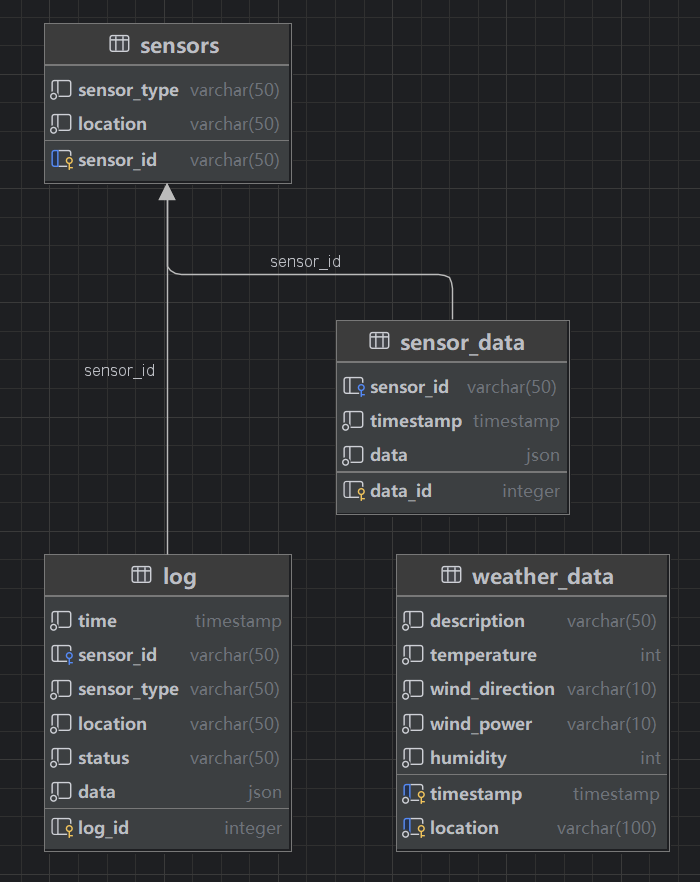
\includegraphics[width=\textwidth]{images/db.png}
    \caption{数据库模式图}\label{db}
\end{figure}

\subsection{数据整合和分析}

我采用Streamlit来构建网页以进行数据整合和分析。所构建的网页分为三部分:主页面、传感器数据展示页面以及传感器日志展示页面,分别如图\ref{Dashboard},图\ref{Data}和图\ref{Log}所示。

\begin{figure}[!htbp]
    \centering
    \includegraphics[width=\textwidth]{images/Dashboard.pdf}
    \caption{主界面}\label{Dashboard}
\end{figure}

\begin{figure}[!htbp]
    \centering
    \includegraphics[height=0.9\textheight]{images/Data.pdf}
    \caption{传感器数据展示界面}\label{Data}
\end{figure}

\begin{figure}[!htbp]
    \centering
    \includegraphics[height=0.9\textheight]{images/Log.pdf}
    \caption{传感器日志展示界面}\label{Log}
\end{figure}